% 3D visualisations of the growth model (20 Oct 2026): stills of the videos in assets/*.mp4 with links.
% Build: pdflatex twice. Rules of CLAUDE.md (supervisor documents): first person singular, no internal labels,
% values not from a paper marked as such, appendix with notation.
\documentclass[aspectratio=169,11pt]{beamer}
\usetheme{Madrid}
\usecolortheme{seahorse}
\usepackage{booktabs}
\usepackage{amsmath,amssymb}
\usepackage{graphicx}
\usepackage{xcolor}
\definecolor{c3}{RGB}{30,80,160}
\setbeamercolor{frametitle}{bg=c3, fg=white}
\setbeamertemplate{navigation symbols}{}
\newcommand{\video}[1]{\href{run:assets/#1}{\scriptsize\textcolor{c3}{$\blacktriangleright$ video: \texttt{\detokenize{assets/#1}}}}}

\title{Biofilm Growth and Stress on a Real Molar}
\subtitle{3D demonstrations of the growth model, with converged stresses and no experimental data}
\author[Keisuke Nishioka]{Keisuke Nishioka}
\institute[IKM, LUH]{\small Institute of Continuum Mechanics (IKM), Leibniz Universit\"at Hannover}
\date{20 October 2026}

\begin{document}
\maketitle

% --------------------------------------------------------
\begin{frame}{What I show}
\small
\begin{itemize}\setlength\itemsep{5pt}
\item Growth model of Klempt et al.\ (2024): phase $\phi$ with $\dot\phi=\beta\nabla^2\phi+k_\alpha\alpha$ (plus the
      bound on $\phi$), growth $\mathbf F_g=\alpha\mathbf I$, stiffness $E(\phi^2+f)$, $E=10$\,Pa, $\nu=0.49$.
\item Added in this work: a nutrient field supplied by the saliva and used up by the biofilm (Klempt et al.\ 2024,
      Eq.~35), and a growth limit by pressure, $\omega=\min\bigl(1,\max(0,1-p/p_h)\bigr)$.
\item Geometry: the thesis's 2\,mm cube for verification, then a real lower first molar at its real size
      (surface from a public CC BY 4.0 data set).
\item Every stress I quote is checked against mesh refinement; values that do not converge are not quoted.
\item Only the verification problem is a thesis result. \textbf{No experimental data are used.}
\end{itemize}
\end{frame}

% --------------------------------------------------------
\begin{frame}{1. Verification: the thesis problem in 3D}
\centering
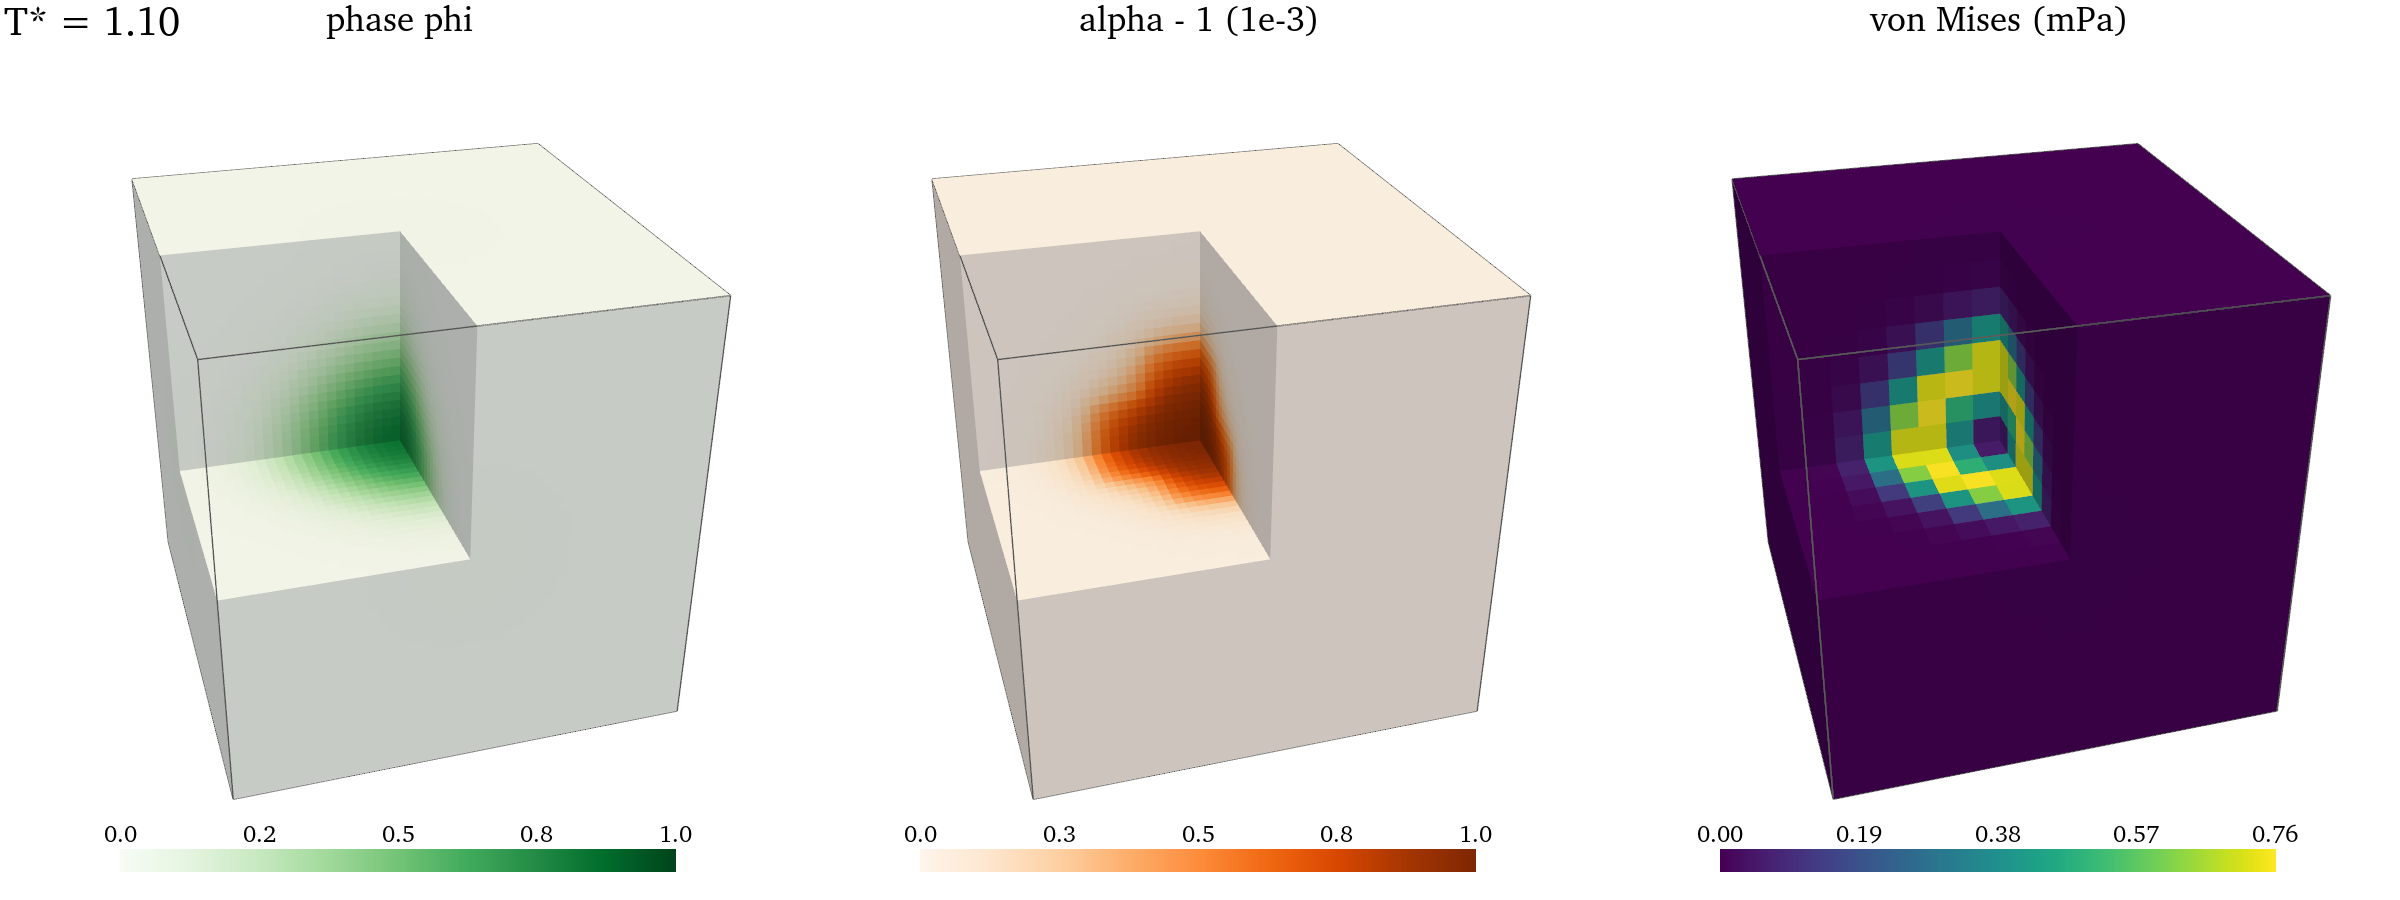
\includegraphics[width=0.9\linewidth]{assets/anim_wp3_seed_3d.png}

\small
$\beta=0.02$\,mm$^2/T^*$, $k_\alpha=10^{-3}/T^*$, $E=10$\,Pa, $\nu=0.49$, $T^*=1.1$; one octant cut away.
Field on $48^3$ (reference solution), stress on $16^3$.\\
Seed von Mises at $T^*=1.1$: $6.19\times10^{-4}$\,Pa (thesis, $16^3$: $6.18\times10^{-4}$\,Pa);
largest value $0.79$\,mPa, converged from $24^3$ on. The stress forms a ring at the edge of the seed.\quad\video{anim_wp3_seed_3d.mp4}
\end{frame}

% --------------------------------------------------------
\begin{frame}{2. Stress next to a fixed surface: what converges}
\centering
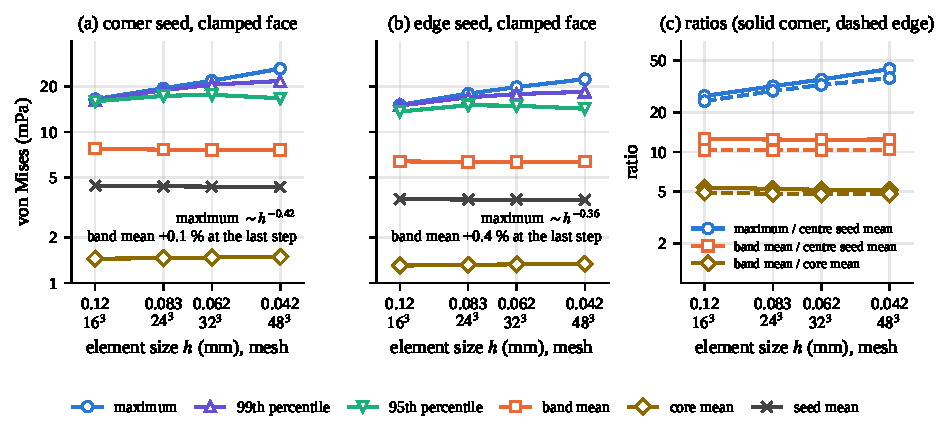
\includegraphics[width=0.9\linewidth,height=0.5\textheight,keepaspectratio]{assets/fig_wall_convergence.pdf}

\small\raggedright
Seed on a clamped face of the cube, meshes $16^3$ to $48^3$. The mean stress in the biofilm next to the face converges
(less than 1\,\% change from $24^3$ on) and is 10 to 12 times the seed stress of the verification problem. The pointwise
maximum, where the clamped face meets a free wall, grows as about $h^{-0.4}$: a corner of the elastic problem.
I quote means and percentiles only.
\end{frame}

% --------------------------------------------------------
\begin{frame}{3. A biofilm on a real molar}
\centering
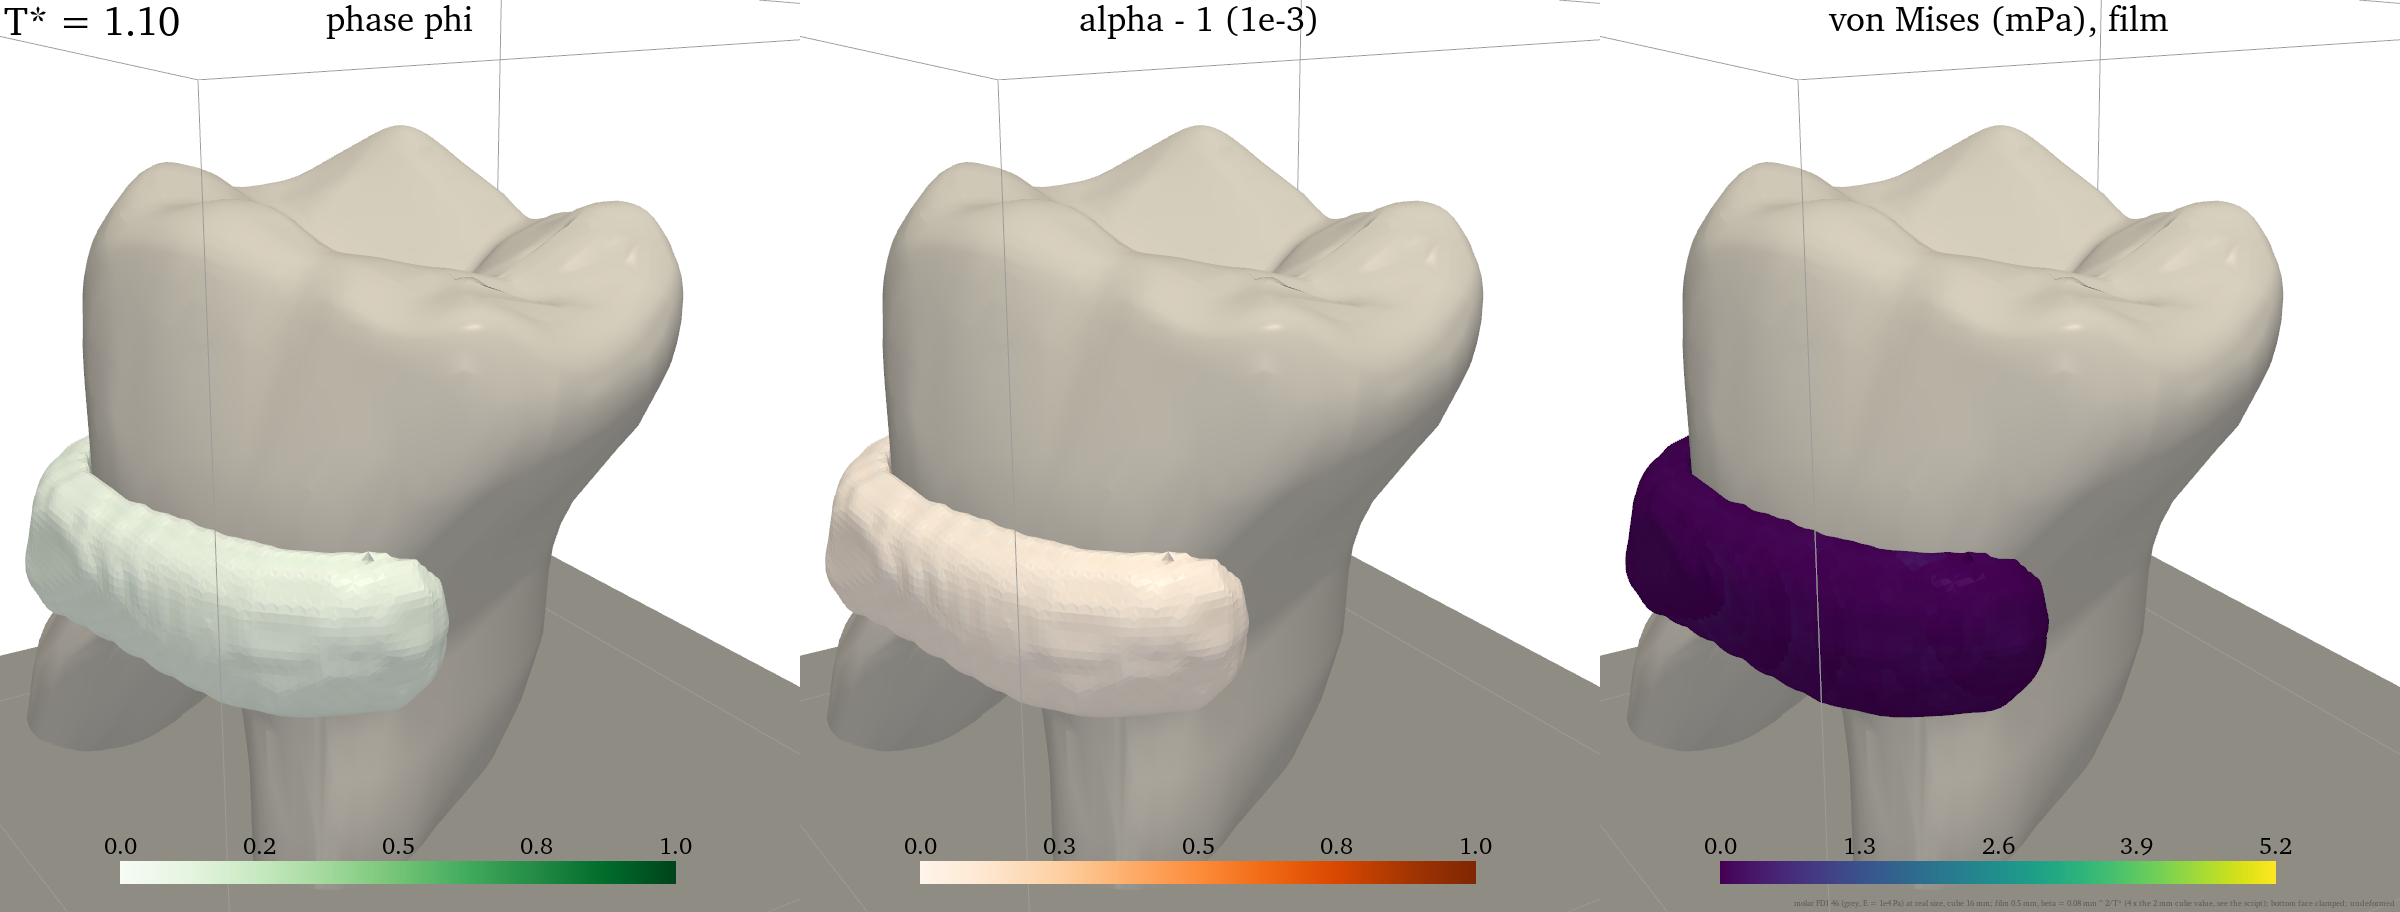
\includegraphics[width=0.92\linewidth]{assets/anim_real_tooth_3d.png}

\small\raggedright
Lower first molar at real size (crown about $10\times12$\,mm) in a 16\,mm box, root clamped. A 0.5\,mm film on one flank
at the cervical third of the crown. $\beta$ is scaled to $0.08$\,mm$^2/T^*$ so that the film spreads by the same share
of its thickness as the thesis seed (an assumption). Growth field converged to 2\,\% ($48^3$ to $192^3$).
\quad\video{anim_real_tooth_3d.mp4}
\end{frame}

% --------------------------------------------------------
\begin{frame}{4. Resolving the stress in a 0.5\,mm film}
\centering
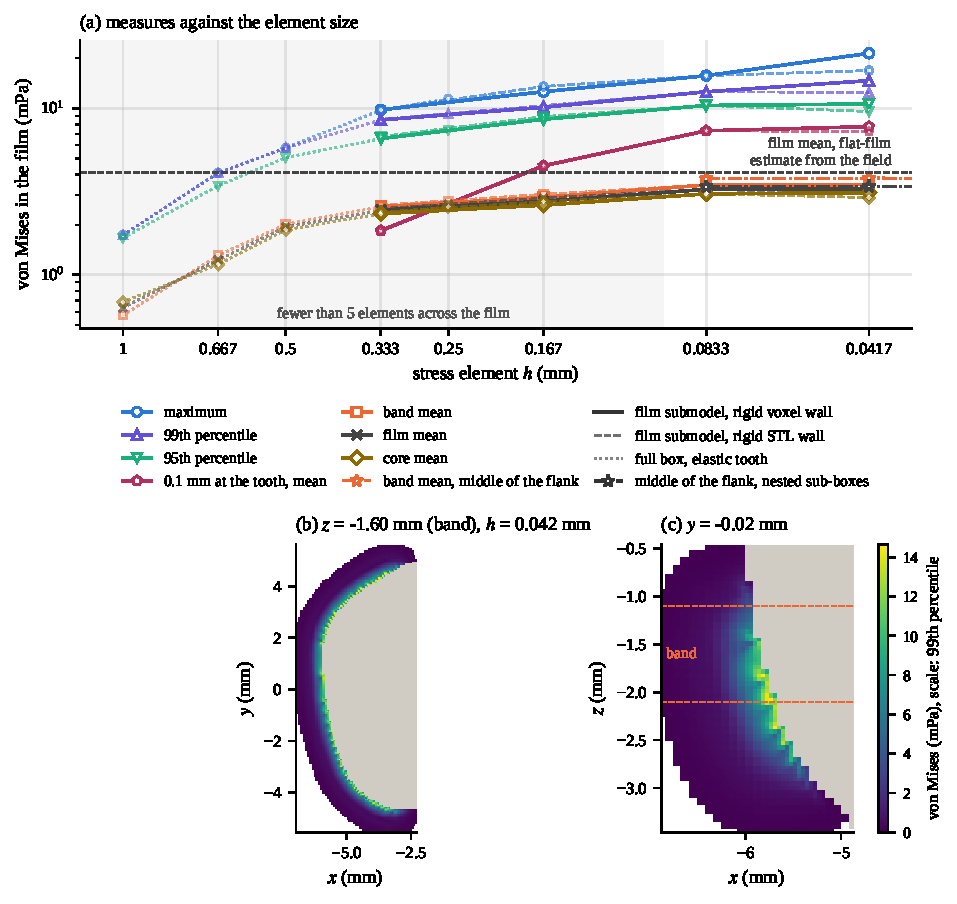
\includegraphics[width=0.9\linewidth,height=0.52\textheight,keepaspectratio]{assets/fig_real_tooth_submodel.pdf}

\small\raggedright
On meshes of the whole box the film is one or two elements thick and the stress does not converge. I solve the film
alone with the tooth as rigid (1000 times stiffer; $0.1\,\%$ effect), down to $h=0.028$\,mm. With six elements across the film
the means converge: film \textbf{3.3\,mPa} ($\pm1\,\%$), cervical band 3.5, the 0.1\,mm next to the tooth 7.8, 95th
percentile 10.5\,mPa. The maximum sits at a corner of the tooth wall and has no converged value.
\end{frame}

% --------------------------------------------------------
\begin{frame}{5. Nutrient and the growth limit on the molar}
\centering
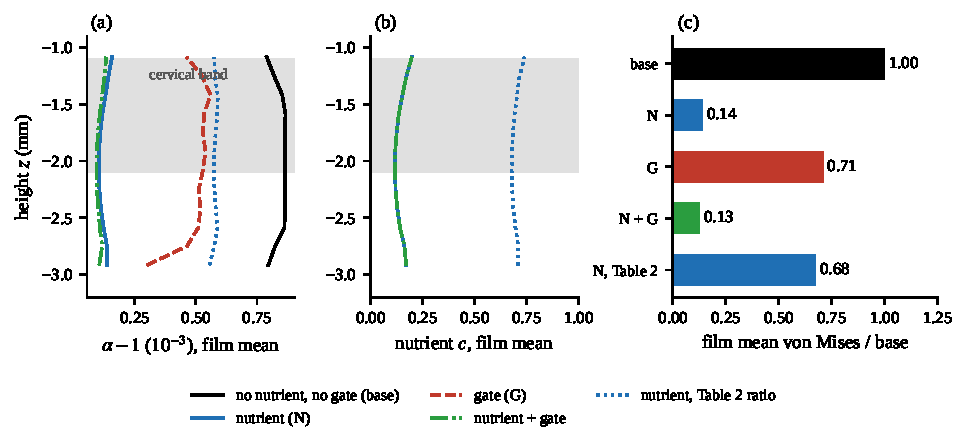
\includegraphics[width=0.88\linewidth,height=0.48\textheight,keepaspectratio]{assets/fig_real_tooth_resolved.pdf}

\small\raggedright
Nutrient from the saliva, consumption $g\phi c$ with $g/d=10$\,mm$^{-2}$ (chosen; 10 times the Table~2 ratio):
$c$ falls to 0.07 at the tooth, and growth and stress drop to about one seventh. At the Table~2 ratio
($c=0.62$ to $0.78$) they drop to 0.68. The growth limit alone ($p_h$ half the film pressure without it, a choice)
gives 0.71; with the nutrient, the nutrient dominates. Stress: end states re-solved with the film model.
\quad\video{anim_real_tooth_nutrient_gate_3d.mp4}
\end{frame}

% --------------------------------------------------------
\begin{frame}{6. Four species on a tooth-like collar (synthetic data)}
\centering
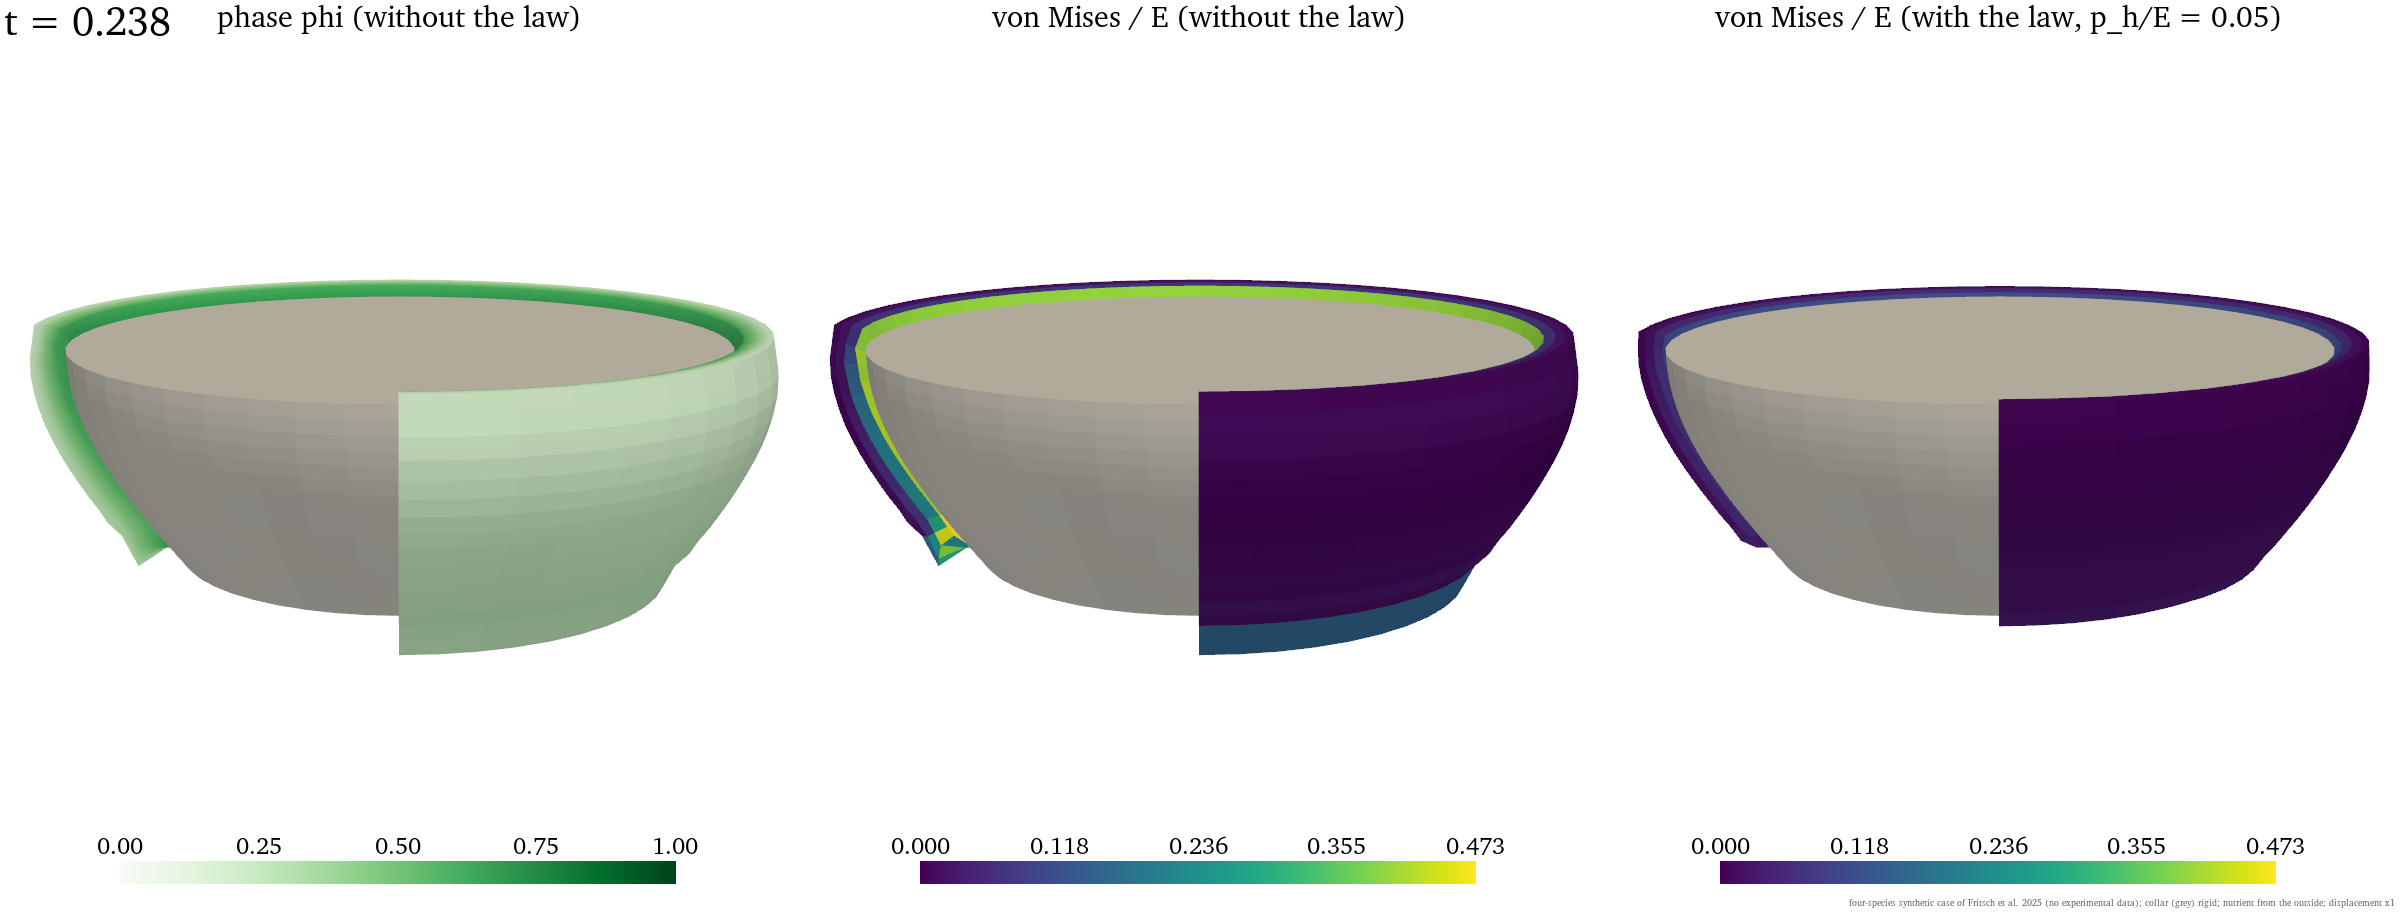
\includegraphics[width=0.93\linewidth]{assets/anim_cervical_f4_3d.png}

\small\raggedright
A 0.25\,mm biofilm layer on a crown-shaped collar (radius 2.05 to 3.05\,mm, 2\,mm high), inner face bonded, nutrient
from the outside. Point model: the four-species case of Fritsch et al.\ (2025) with their true parameters
(synthetic, no experimental data). One quarter is cut away. Growth is large here (displacement up to 0.31\,mm),
drawn at true scale.\quad\video{anim_cervical_f4_3d.mp4}
\end{frame}

% --------------------------------------------------------
\begin{frame}{6. Section and composition}
\centering
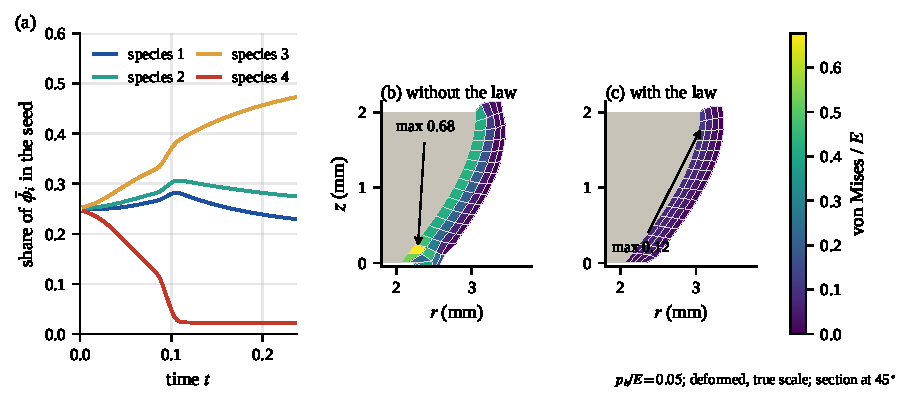
\includegraphics[width=0.82\linewidth]{assets/fig_cervical_f4.pdf}

\small\raggedright
(a) Species 3 takes over the seed (share 0.47 at the end), species 4 almost disappears (0.02).
(b), (c) Section at $45^\circ$: without the law the von Mises stress reaches $0.68E$ at the bonded base;
with $p_h/E=0.05$ the largest value is $0.12E$.
\end{frame}

% --------------------------------------------------------
\begin{frame}{Summary}
\small
\begin{itemize}\setlength\itemsep{6pt}
\item The 3D view reproduces the thesis value of the seed stress (0.2\,\% difference).
\item Next to a fixed surface the biofilm stress is 10 to 12 times the free-seed value (converged band mean);
      pointwise maxima at corners have no converged value.
\item On a real molar, a 0.5\,mm film needs about six elements across it; then the film mean is 3.3\,mPa
      ($E=10$\,Pa), highest in the 0.1\,mm next to the tooth (2.4 times the mean).
\item A nutrient limited by consumption lowers growth and stress more than the pressure limit; the pressure limit
      removes stress concentrations in the cube and on the collar.
\item Next at Keio: the calibrated parameters of Chapter~3 on this molar, the gate with the film stress in every step,
      and an implant.
\end{itemize}
\end{frame}

% --------------------------------------------------------
\appendix
\begin{frame}{Appendix A: notation and equations}
\small
\begin{tabular}{@{}ll@{}}
\toprule
$\phi$ & biofilm phase (volume fraction) \\
$\alpha$ & growth, $\mathbf F_g=\alpha\mathbf I$, $\alpha(0)=1$; growth is $\alpha-1$ \\
$\beta$, $k_\alpha$ & diffusion of $\phi$, growth rate (Klempt et al.\ 2024, Eq.\ 34/36) \\
$E(\phi^2+f)$ & stiffness, $f=10^{-3}$ (void) \\
$p$, $p_h$, $\omega$ & pressure $-\tfrac13\operatorname{tr}\boldsymbol\sigma$, homeostatic pressure, growth limit \\
$c$, $d$, $g$ & nutrient, its diffusion, consumption rate (Klempt et al.\ 2024, Eq.\ 35) \\
$\phi_i,\psi_i,\bar\phi_i=\phi_i\psi_i$ & point model (Klempt et al.\ 2026): volume fraction, living fraction \\
$c^*$ & nutrient scale of the point model (25 in the four-species case) \\
\bottomrule
\end{tabular}

\vspace{6pt}
Cube and molar: $\dot\phi=\beta\nabla^2\phi+k_\alpha\alpha-P\,[\max(0,\phi-1)+\min(0,\phi)]$, $P=5$;
$\dot\alpha=k_\alpha\phi\,c\,\omega$ ($c=1$ without the nutrient, $\omega=1$ without the limit).\\
Collar: growth from the point model in the element of this work, scaled by the same $\omega$.
\end{frame}

\begin{frame}{Appendix B: sources}
\small
\begin{itemize}\setlength\itemsep{5pt}
\item Tooth surface: C.~Diaz, C.~A.~Ferro S\'anchez, O.~Campo, \emph{Data of synthetic 3D models of the human jaw,
      including teeth, ligaments, and bone structures}, Mendeley Data V1 (2024), doi:10.17632/xjsx7nfhj8.1,
      licence CC BY 4.0; file \texttt{D46.stl} (lower right first molar), used unchanged.
\item Growth model and parameters: F.~Klempt et al., Biomech.\ Model.\ Mechanobiol.\ (2024).
\item Four-species synthetic case: L.~Fritsch et al., arXiv:2512.15145 (2025), Case II, true parameters.
\item Scripts and reports: \texttt{ansys\_usermat/apdl/} (\texttt{real\_tooth\_*.py}, \texttt{results/2026-10-3d/}).
\end{itemize}
\end{frame}

\begin{frame}{Appendix C: settings}
\footnotesize\setlength{\tabcolsep}{4pt}
\begin{tabular}{@{}llll@{}}
\toprule
case & geometry & mesh (field / stress) & values \\
\midrule
verification & 2\,mm cube, seed in the centre & $48^3$ / $16^3$ & thesis (Ch.\ 4) \\
wall study & cube, seed on a clamped face & $96^3$ / $16^3$--$48^3$ & thesis values \\
real molar & 16\,mm box, film 0.5\,mm & $96^3$, $192^3$ / film model to 0.028\,mm & $\beta$ scaled $\times4$ \\
nutrient, limit & real molar & $96^3$ / film model 0.083\,mm & $g/d$ and $p_h$ chosen \\
collar & quarter ring, $4\times12\times16$ & element of this work & Fritsch et al.\ 2025 \\
\bottomrule
\end{tabular}

\vspace{6pt}
Small strain, hex8 with B-bar in the cube and on the molar (rigid tooth, $E_{\rm tooth}=10^4$\,Pa where elastic);
finite strain on the collar. Growth with the nutrient: $\dot\alpha=k_\alpha\phi c\,\omega$ (the factor $c$ is an
assumption; Eq.~36 as printed has none). Nutrient quasi-static, $0=d\nabla^2c-g\phi c$, $c=1$ at the saliva.
\end{frame}
% --------------------------------------------------------
\begin{frame}{Backup: seed in a corner and on an edge (cube)}
\centering
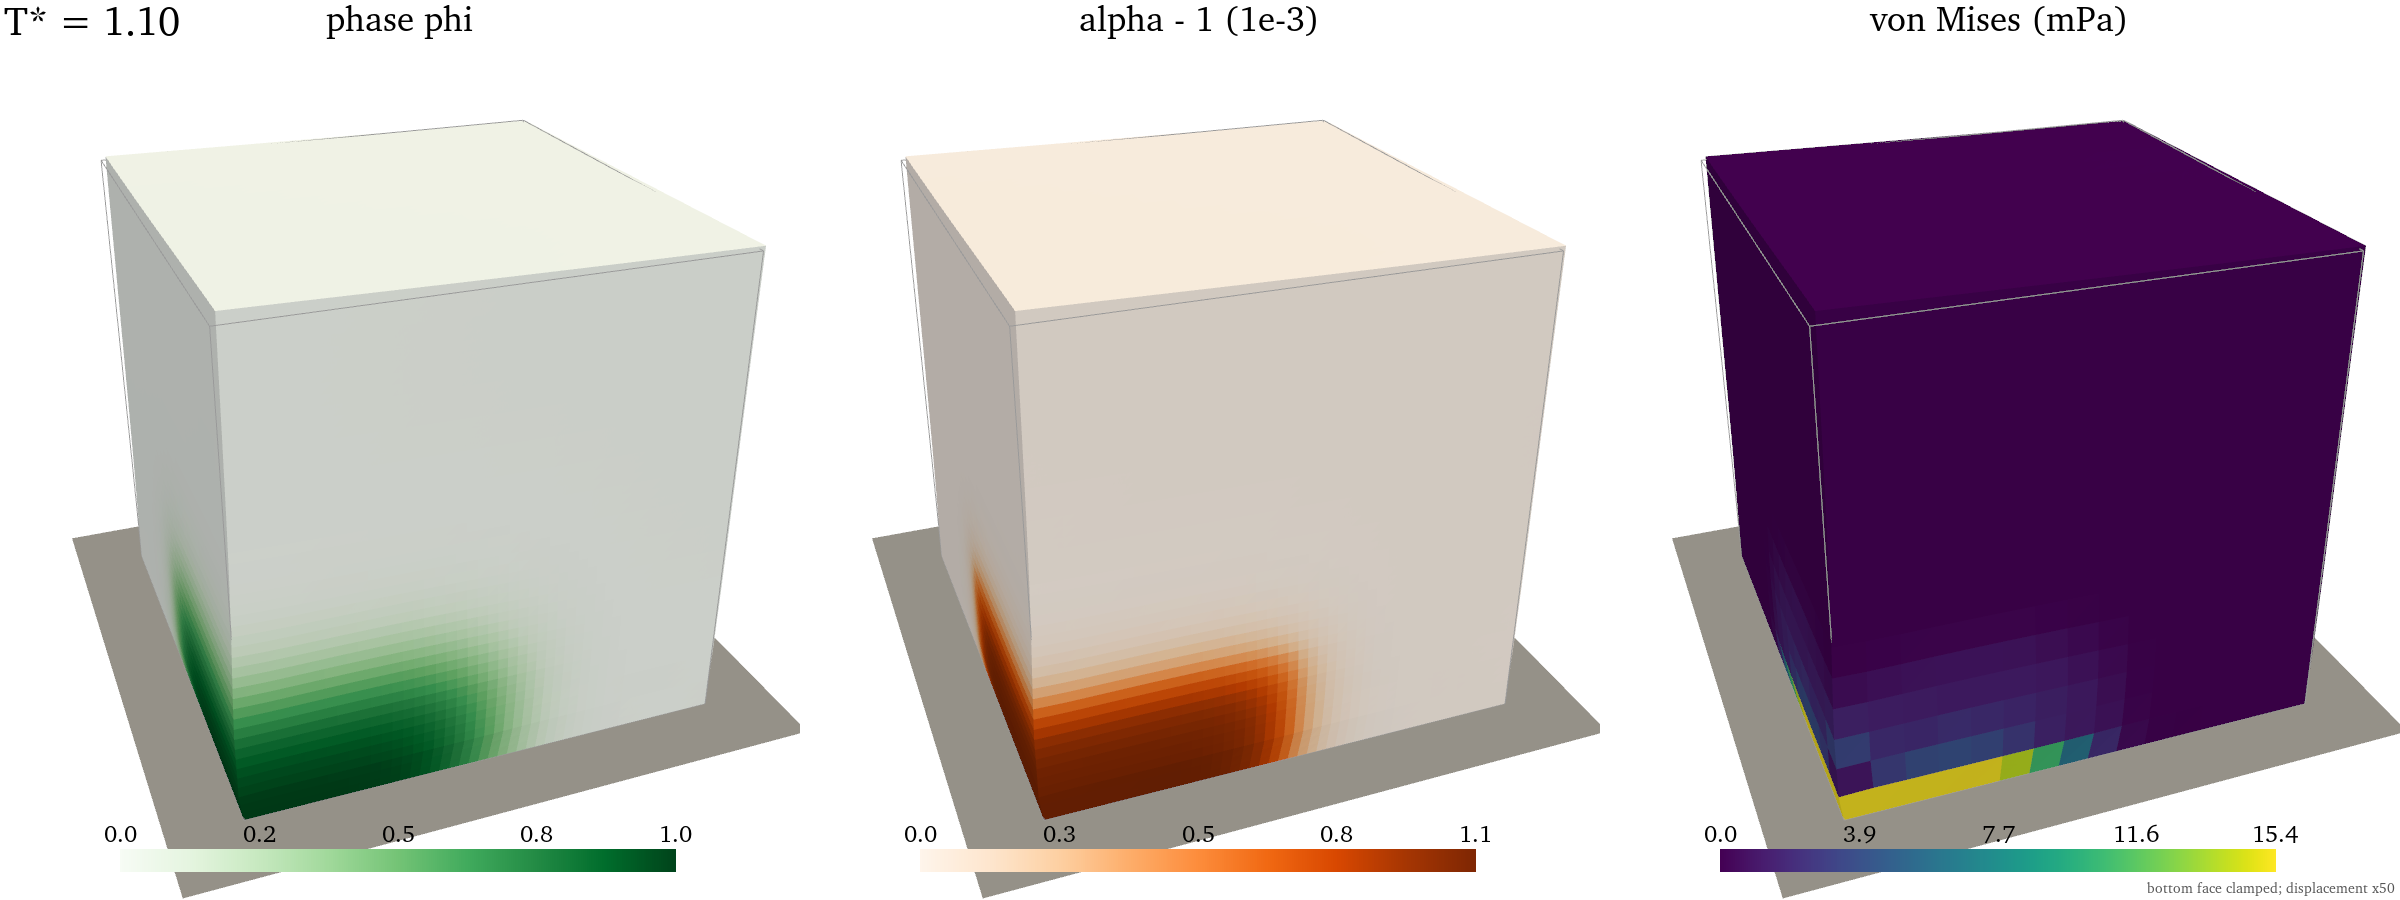
\includegraphics[width=0.49\linewidth]{assets/anim_seed_corner_3d.png}\hfill
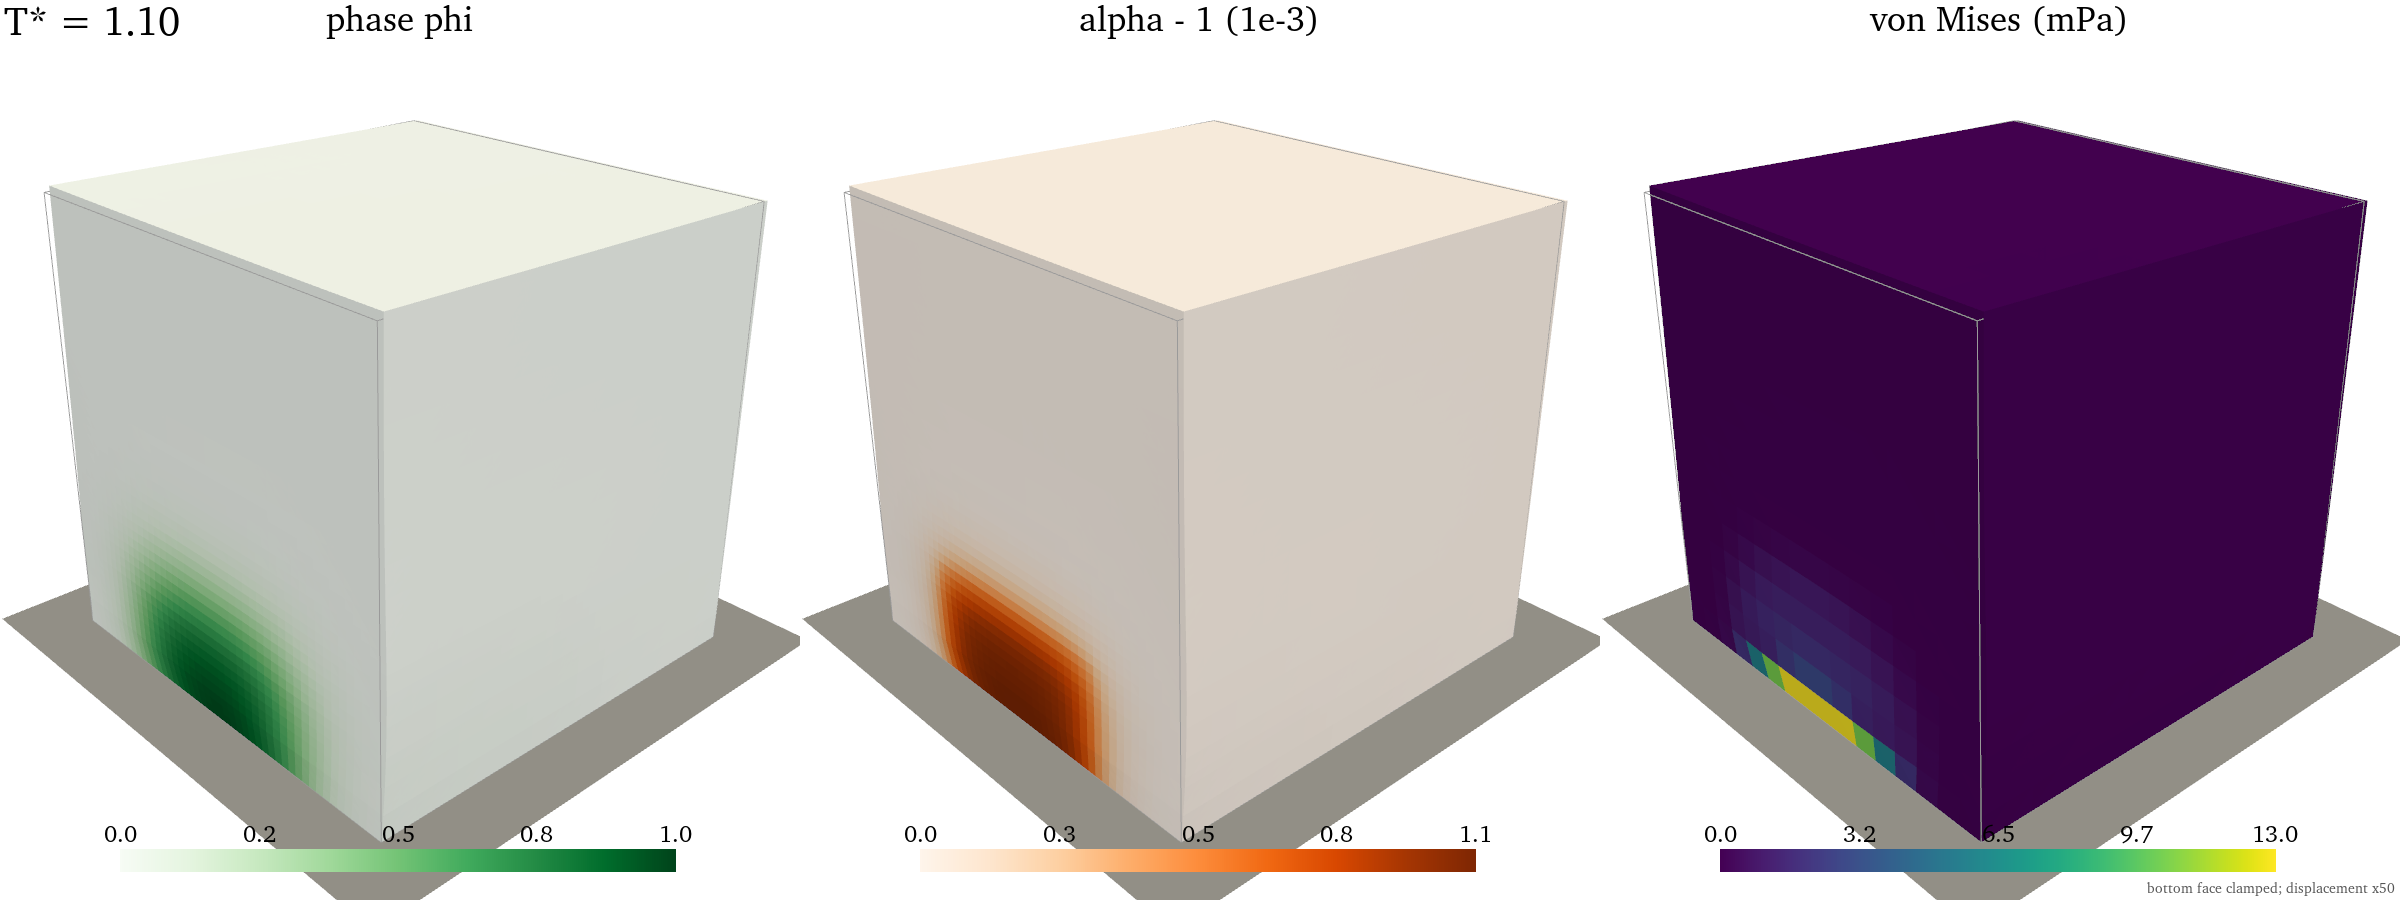
\includegraphics[width=0.49\linewidth]{assets/anim_seed_edge_3d.png}

\small\raggedright
Same model and seed volume as the verification problem; bottom face clamped (the substrate). Left: corner (three faces), right: edge
(two faces). The biofilm spreads along the walls; the stress concentrates in the biofilm next to the clamped face: the mean over
its bottom quarter millimetre is 7.6\,mPa (corner) and 6.4\,mPa (edge), 10 to 12 times the seed stress of the centre
case (0.61\,mPa) and about 5 times the mean of the layer above it; these means change by less than 1\,\% from
$24^3$ to $48^3$. The pointwise maximum sits where the clamped face meets a free wall and grows with refinement
(16 to 26\,mPa, about $h^{-0.4}$), so the colour scale stops at the 95th percentile, about 15\,mPa, which does not
depend on the mesh.\\
\video{anim_seed_corner_3d.mp4}\quad\video{anim_seed_edge_3d.mp4}
\end{frame}

% --------------------------------------------------------
\begin{frame}{Backup: two seeds that grow into each other (cube)}
\centering
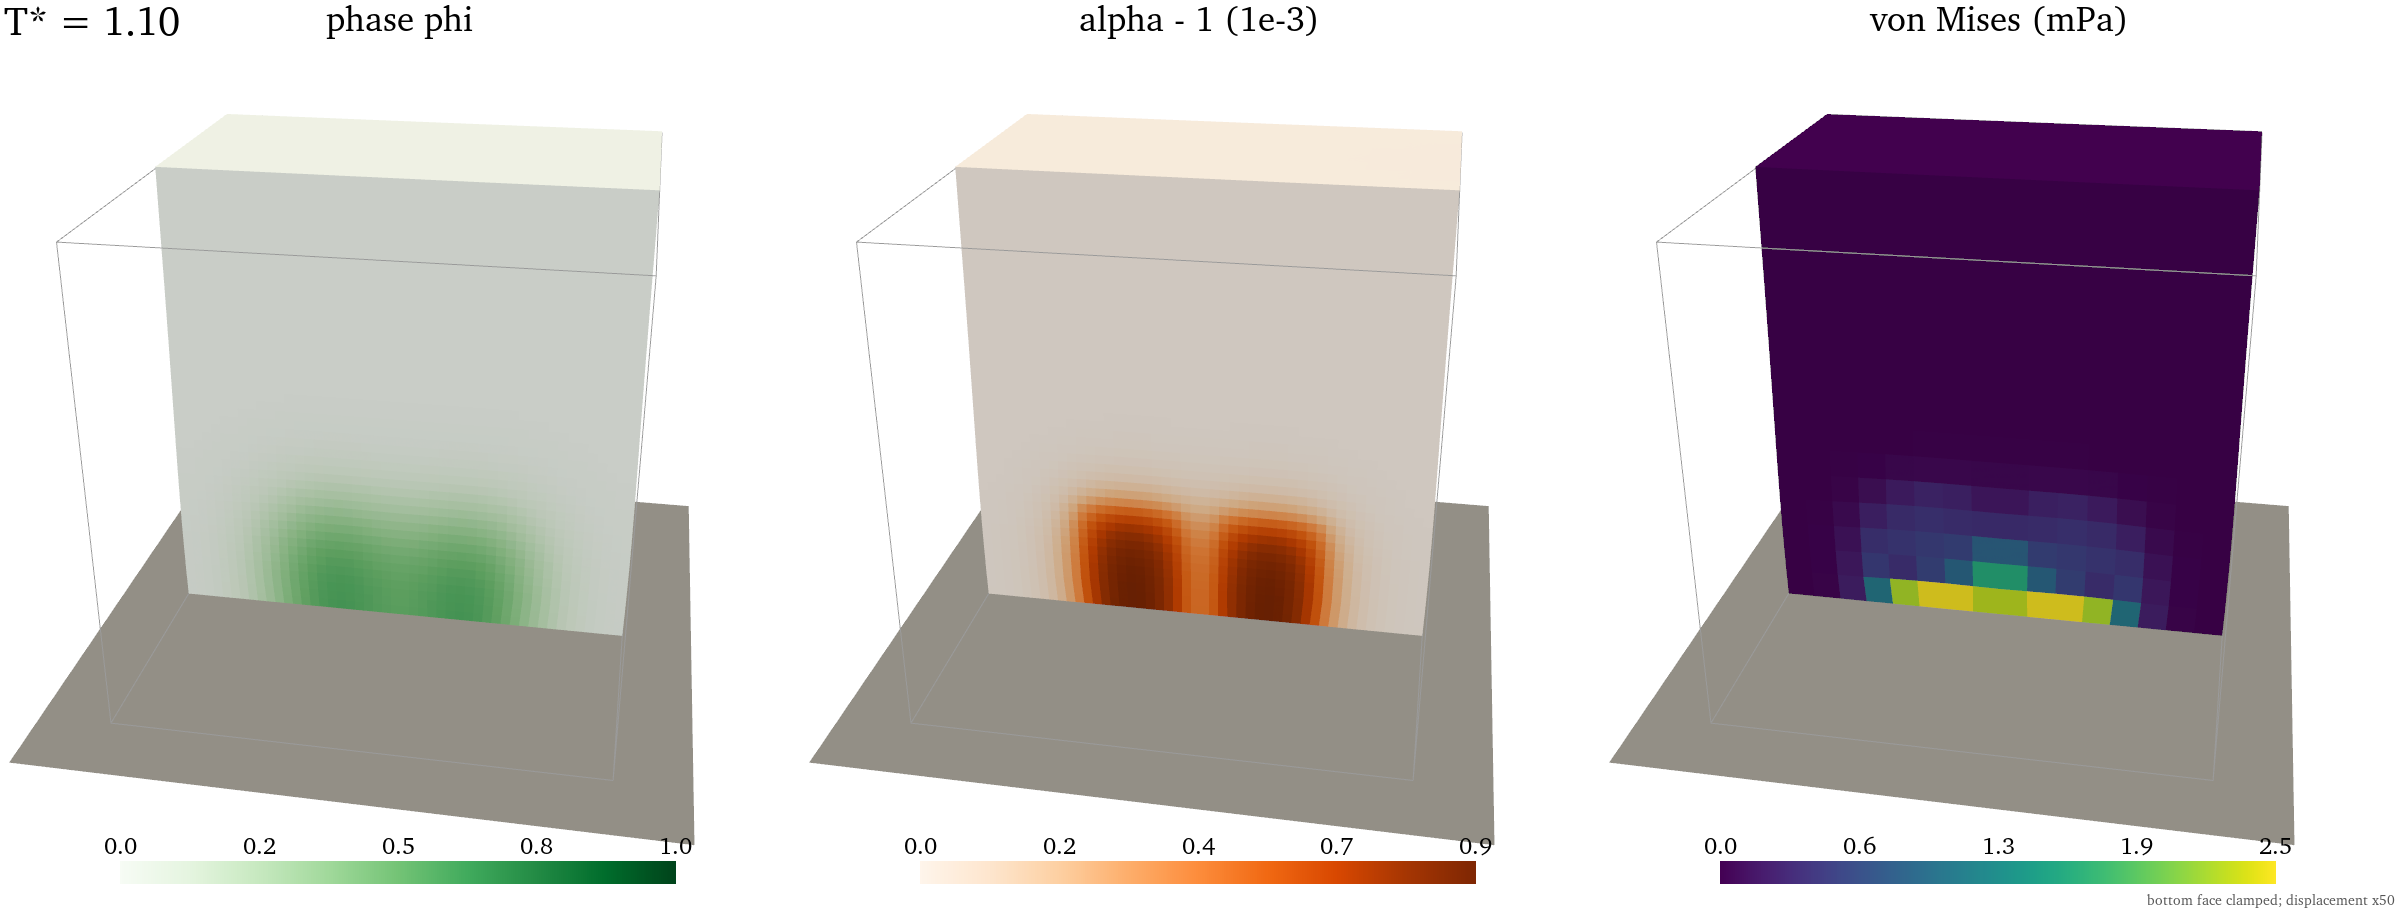
\includegraphics[width=0.95\linewidth]{assets/anim_two_3d.png}

\small\raggedright
Two seeds of 0.5\,mm on the clamped bottom face, 0.125\,mm apart; front half cut away; same model as the verification problem.
The two seeds join, and the stress is highest along the clamped face under both of them.\quad\video{anim_two_3d.mp4}
\end{frame}

% --------------------------------------------------------
\begin{frame}{Backup: the growth limit in the cube}
\centering
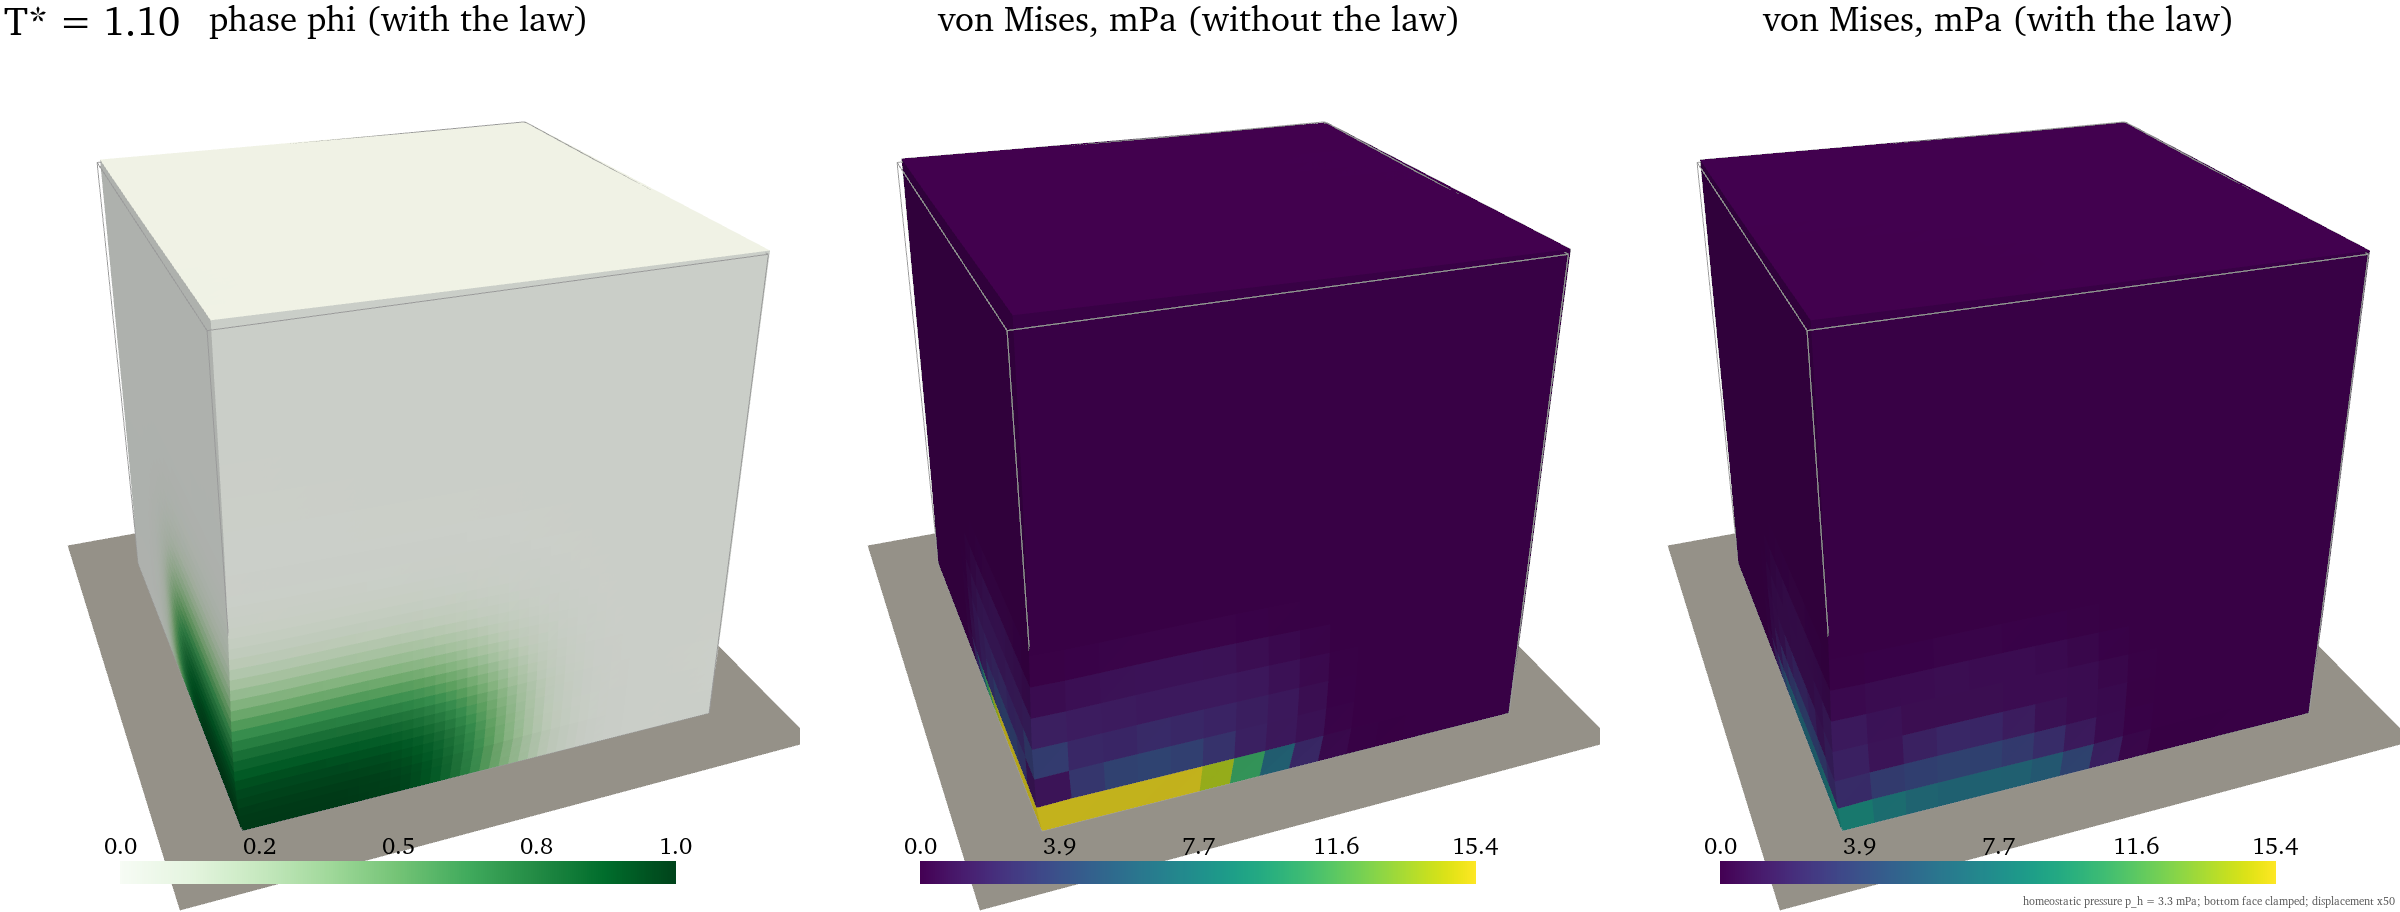
\includegraphics[width=0.95\linewidth]{assets/anim_law_3d.png}

\small\raggedright
Corner seed, same colour scale in both stress panels. Without the law the stress in the biofilm next to the clamped
face reaches about 15\,mPa (95th percentile, the top of the colour scale); with the law it stays well below. $p_h=3.3$\,mPa is chosen by me (0.4 times the 95th percentile of the
pressure without the law), not taken from a paper.\quad\video{anim_law_3d.mp4}
\end{frame}

\end{document}
